\section{Track Selection}\label{section:star_track_selection}
The following quality cuts had to be passed by the selected primary tracks in this analysis:
\begin{enumerate}
	\item The tracks must be matched with hits reconstructed in TOF,
	\item The number of the  TPC hits used in the helix fit $N_{\textrm{hits}}^{\textrm{fit}}$ must be greater than $24$,
	\item The~ratio of $N_{\textrm{hits}}^{\textrm{fit}}$ to the~number of all possible TPC hits, $N_{\textrm{hits}}^{\textrm{fit}}/N_{\textrm{hits}}^{\textrm{possible}}$, must be greater than $0.52$,
	\item The number of the  TPC hits used to determine the $dE/dx$ information $N_{\textrm{hits}}^{\textrm{dE/dx}}$ must be greater than $14$,
	\item The transverse impact parameter with respect to the beamline $d_0$ must be less than $1.5$~cm,
	\item The radial component of the distance of the closest approach between  the global helix and the vertex $\textrm{DCA}_{xy}$ must be less than $1.5$~cm (consistent with the $d_0$ limit),
	\item The absolute magnitude of  longitudinal component of the distance of the closest approach between  the global helix and the vertex $|\textrm{DCA}_{z}|$ must be less than $1$~cm,
	\item The track's transverse momentum $p_\textrm{T}$ must be greater than $0.2$~GeV/c,
	\item The track's absolute value of  pseudorapidity $|\eta|$ must be smaller than $0.7$.
\end{enumerate}

\begin{figure}[b!]
	\centering
	\begin{subfigure}{.45\textwidth}
		\includegraphics[width=\textwidth, page=8]{chapters/chrgSTAR/img/selection/SDT.pdf}
		\caption{}
	\end{subfigure}
	\begin{subfigure}{.45\textwidth}
		\includegraphics[width=\textwidth, page=7]{chapters/chrgSTAR/img/selection/SDT.pdf}
		\caption{}
	\end{subfigure}
	\begin{subfigure}{.45\textwidth}
		\includegraphics[width=\textwidth, page=3]{chapters/chrgSTAR/img/selection/SDT.pdf}
		\caption{}
	\end{subfigure}
	\begin{subfigure}{.45\textwidth}
		\includegraphics[width=\textwidth, page=4]{chapters/chrgSTAR/img/selection/SDT.pdf}
		\caption{}
	\end{subfigure}
	\begin{subfigure}{.45\textwidth}
		\includegraphics[width=\textwidth, page=9]{chapters/chrgSTAR/img/selection/SDT.pdf}
		\caption{}
	\end{subfigure}
	\begin{minipage}{.45\textwidth}
		
		
		\caption{Number of the  TPC hits used in the helix fit (a) and number of the  TPC hits used to determine the $dE/dx$ (b), the radial component (c) and the absolute magnitude of the longitudinal component (d) of the distance of the closest approach between  the global helix and the vertex, transverse impact parameter w.r.t. beam-line (e). All distributions are shown before applying  the corresponding cuts. Blue lines indicate regions accepted in the analysis.}
		\label{fig:dca_nhitsSTAR}
	\end{minipage}
\end{figure}

\begin{figure}[h!]
	\centering
	\begin{subfigure}{.45\textwidth}
		\includegraphics[width=\textwidth, page=2]{chapters/chrgSTAR/img/selection/SDT.pdf}
		\caption{}
	\end{subfigure}
	\begin{subfigure}{.45\textwidth}
		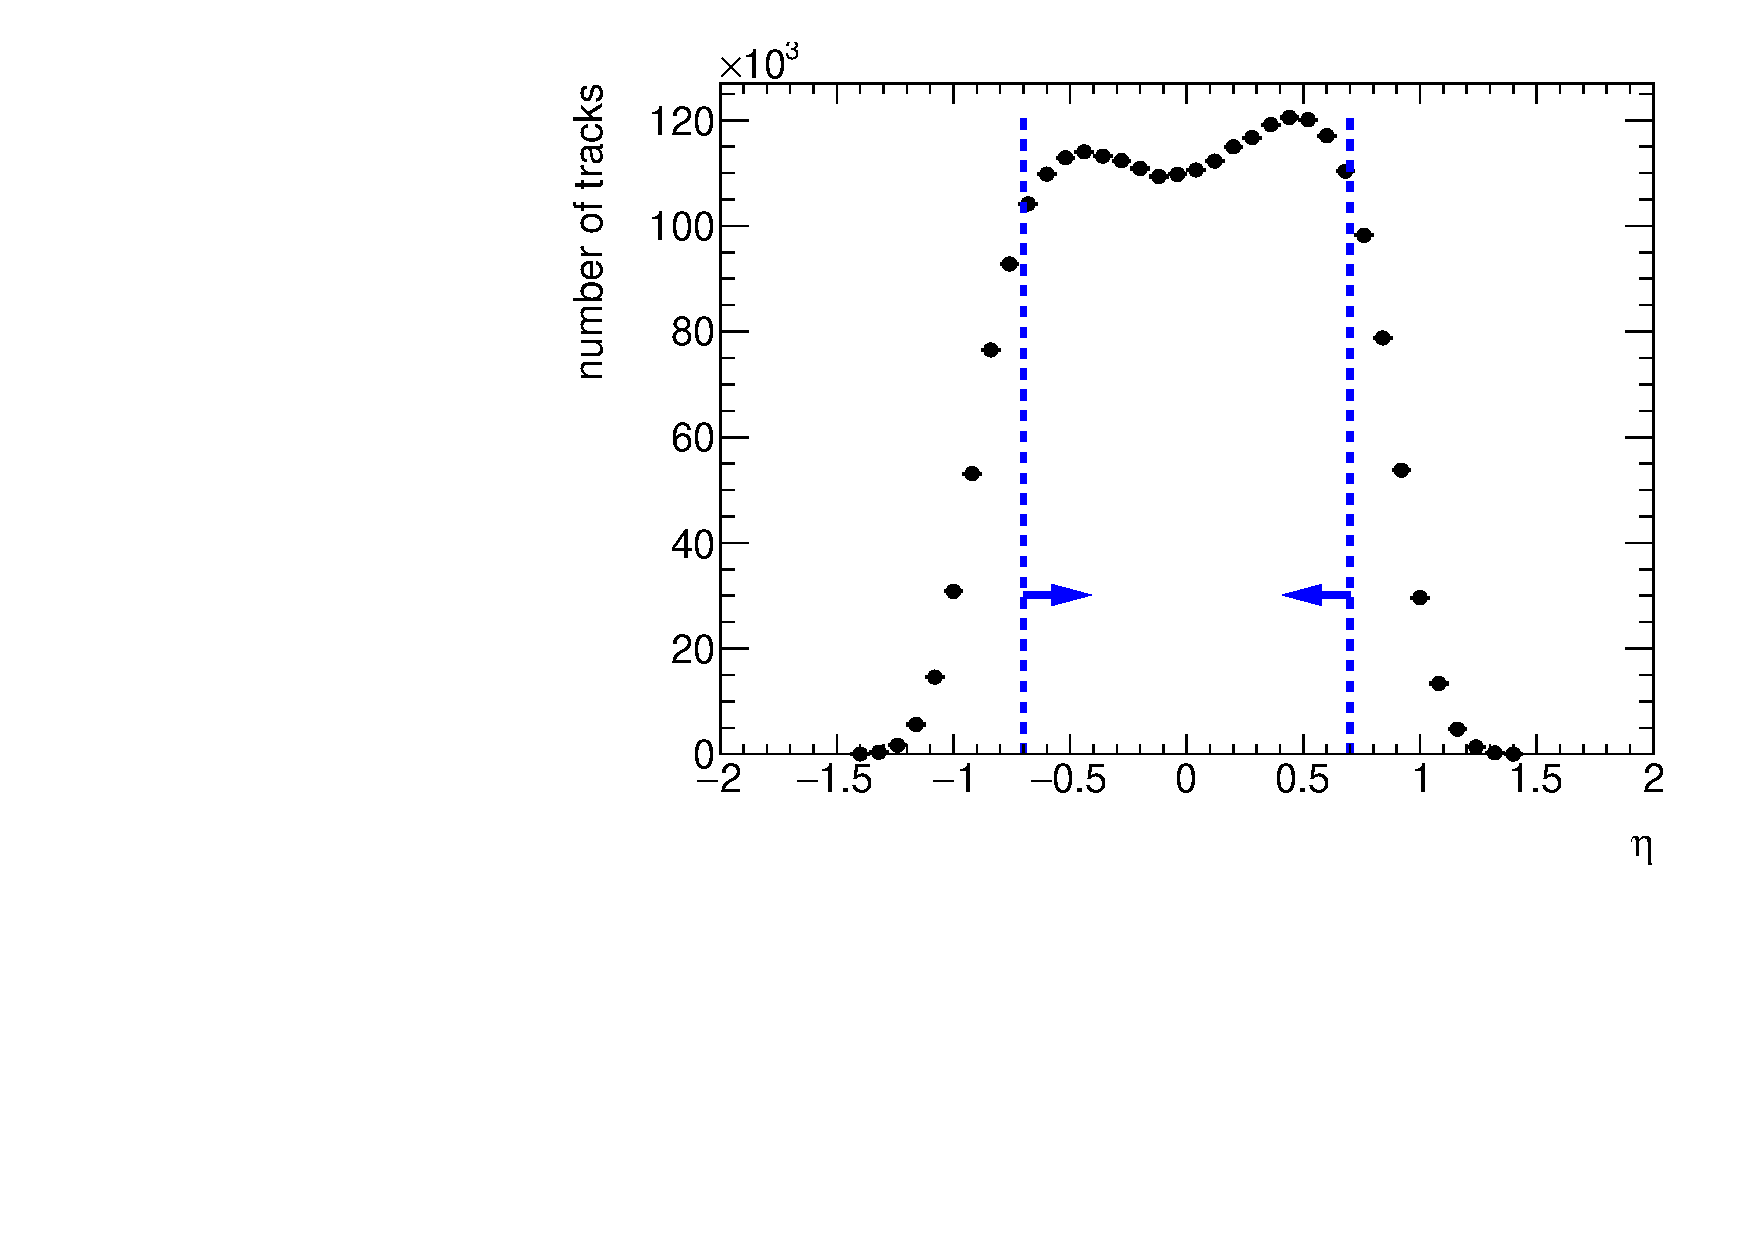
\includegraphics[width=\textwidth, page=1]{chapters/chrgSTAR/img/selection/SDT.pdf}
		\caption{}
	\end{subfigure}
	\begin{subfigure}{.45\textwidth}
		\includegraphics[width=\textwidth, page=10]{chapters/chrgSTAR/img/selection/SDT.pdf}
		\caption{}
	\end{subfigure}
	\begin{minipage}{.45\textwidth}
		
		
		\caption{Transverse momentum (a), pseudorapidity (b) and azimuthal angle (c) of the~reconstructed tracks. All distributions are shown before applying  the corresponding cuts. Blue lines indicate regions accepted in the analysis.}
		\label{fig:ptEtaPhiSTAR}
	\end{minipage}
\end{figure}


The $N_{\textrm{hits}}^{\textrm{fit}}$ and $N_{\textrm{hits}}^{\textrm{fit}}/N_{\textrm{hits}}^{\textrm{possible}}$ cuts are used to reject low quality TPC tracks and avoid track splitting effects. The $d_0$ and global $\textrm{DCA}_{xy}$,  $|\textrm{DCA}_{z}|$ cuts are used to select tracks that originate from the primary interaction vertex. The cut on $N_{\textrm{hits}}^{\textrm{dE/dx}}$ is used to ensure that selected tracks have sufficient energy loss information
for particle identification purposes. In this analysis tracks without identification are required to have $p_\textrm{T} > 0.2$~GeV/c and $|\eta| < 0.7$ due to high track reconstruction and TOF matching efficiencies in this region. For the identified particle-antiparticle ratio analysis, where in addition to charged pions, charged kaons and (anti)proton  are measured, the $p_T$ cut was increased  to $0.3$ and $0.4$~GeV/c, respectively. 
The distributions of the $\textrm{DCA}_{xy}$, $|\textrm{DCA}_{z}|$, $d_0$, $N_{\textrm{hits}}^{\textrm{fit}}$ and $N_{\textrm{hits}}^{\textrm{dE/dx}}$ quatities together with applied cuts are shown in Fig.~\ref{fig:dca_nhitsSTAR}, while the~$p_T$, $\eta$ and  the~azimuthal angle, $\phi$, of the~reconstructed tracks are shown in Fig.~\ref{fig:ptEtaPhiSTAR}. Data are compared to embedded PYTHIA~8 SD sample.



